\chapter{Algoritmos de generaci\'on de datos de prueba}
En el desarrollo de un software que hace uso de una base de datos es muy importante para los desarrolladores sobre todo para los que son encargados de la base de datos, trabajar con una base de datos con datos de prueba  que se asemejen m\'as a las reales tanto en cantidad como en tipo de datos, para lo cual es necesario tener una cantidad grande de datos de prueba cuanto m\'as mejor, esto lleva a un enfoque de generar datos de prueba para base de datos.


Poseer con una cantidad suficiente de datos de prueba no es tan sencillo por lo que un desarrollador normalmente acostumbra hacer la inserci\'on de forma manual lo cual toma un  tiempo excesivo. Ademas cuando se quiere hacer la inserci\'on es necesario tener en cuenta los diferentes tipos de datos que la gran mayor\'ia de los SGBD (\texttt{Sistemas gestor de base de datos}) posee.
 
Los tipos de datos que manejan los SGBD mediante SQL permiten definir el formato de la informaci\'on a usar en  columnas, variables y expresiones. Cabe aclarar que dependiendo del SGBD a usarse los tipos de datos pueden cambiar.

Al igual que otros lenguajes de programaci\'on, para SQL se puede encontrar n\'umeros enteros, flotantes, cadenas, booleanos y dem\'as. entre los mas utilizados se tiene:

\begin{itemize}
\item Tipos de datos flotantes para representar numero de punto flotante (\texttt{float, real}).
\item Tipos de datos temporales es seguro que en alg\'un momento es necesario guardar registros que contengan informaci\'on sobre fechas de cumplea\~nos, tiempo de llegada. Para este caso existen tipos de datos(\texttt{date,datetime,timestamp,time}).
\item Cadenas de caracteres, guardar nombres, apellidos, direcciones y otros tipos de datos denominativos requiere que el uso de cadenas de caracteres para lo cual se tiene tipos de datos (\texttt{char,varchar,text}).
\end{itemize}

\begin{center}
  \scriptsize	
  \captionof{table}{Tipos de datos}
  \label{tablaTipoDatos1} % for use in \ref{table1} if you want to refer to the table number
  \renewcommand{\arrayrulewidth}{1pt}
\begin{tabular}{|p{40mm}|p{98mm}|}\hline
\textbf{Tipo de dato} & \textbf{Caracter\'isticas}\\\hline
\texttt{VARCHAR}(tama\~no) & Almacena cadenas de caracteres de una longitud variable.
La longitud m\'axima son 4000 caracteres \\\hline
\texttt{CHAR}(tama\~no)&
Almacena caracteres con una longitud fija. Siendo 2000 caracteres el m\'aximo\\\hline
\texttt{NUMBER}(precisi\'on, escala) &
Almacena datos num\'ericos, tanto enteros como decimales, con o sin signo. Precisi\'on, indica el n\'umero m\'aximo de d\'igitos que va a tener el dato. Escala, indica el n\'umero de d\'igitos que puede haber a la derecha del punto decimal.\\\hline
\texttt{LONG}&
Almacena cadenas de caracteres de longitud variable. Puede almacenar hasta 2 gigas de informaci\'on\\\hline
\texttt{LONG RAW}&
Almacena datos binarios. Se emplea para el almacenamiento de gr\'aficos, sonidos, etc. Su tama\~no m\'aximo es de 2 gigas\\\hline
\texttt{DATE} &
Almacena informaci\'on de fechas y horas. De forma predeterminada almacena un dato con el siguiente formato: siglo/a\~no/mes/dia/hora/minutos/segundos. Este formato se puede cambiar con otros par\'ametros.\\\hline
\texttt{RAW}(tama\~no)&
Almacena datos binarios. Puede almacenar como mucho 2000 bytes.\\\hline
\texttt{ROWID}&
Se trata de un campo que representa una cadena hexadecimal que indica la direcci\'on de una fila en su tabla\\\hline
\texttt{NVARCHAR2}(tama\~no)&
Es similar al varchar2 pero el tama\~no de un car\'acter depende de la elecci\'on del juego de caracteres. El tama\~no m\'aximo es 2000 bytes.\\\hline
\texttt{NCHAR}(tama\~no)&
Similar al \texttt{CHAR} y con las mismas caracter\'isticas que el \texttt{nvarchar2}\\\hline
\texttt{CLOB}&
Similar al \texttt{LONG} y se usa para objectos car\'acter\\\hline
\texttt{BLOB} &
Similar al \texttt{LONG RAW}. Este se usa para objetos binarios.\\\hline
\end{tabular}
\end{center}
\section{Algoritmos de generaci\'on de datos}
La generaci\'on de datos de prueba para base de datos no llega a ser tan sencilla por los diferentes tipos de datos y el l'imite en el tama\~no, pero llega a ser una soluci\'on  para pruebas que se quiera realizar a una base de datos determinada. Para realizar la generaci\'on de datos  es necesario tener algoritmos generadores por cada tipo de datos que tome en cuenta las caracter\'isticas de la misma  y sean capaces de generar cantidades grandes tomando como base una peque\~na cantidad de datos o a lo mejor sin contar ninguna base.
\section{Tipos num\'ericos}
Existen varios tipos de datos para manejar n\'umeros enteros dentro de \texttt{SQL}. Todas esas opciones se diferencian en el tama\~no de memoria asignado para un rango de valores enteros.

Los n\'umeros enteros es uno de los m\'as sencillos a generar, con solo incrementar en una unidad al n\'umero  inicial que se pasa como par\'ametro se llega en alg\'un momento al l\'imite que tambi\'en se pasa como par\'ametro.
\section{Tipos monetarios}
Los tipos de datos monetarios se almacenan como un numero cualquiera y tiene una similitud con las decimales, el SGBD es quien se encarga de dar el formato necesario. 
\section{Tipos de caracteres}
\subsection{Generaci\'on de nombres}
El generar nombres se puede hacer de varias formas en este proyecto se muestra dos maneras: a partir de una lisata de nombres y apellidos  o tambi\'en se puede generar haciendo combinaciones de las vocales y las consonantes, a continuaci\'on se har\'a una descripci\'on de c\'omo generar de las dos formas.
\subsubsection{Generaci\'on de nombres a partir de vocales y consonantes}
Un nombre se compone generalmente por m\'as de tres caracteres puede que tenga menos y a lo mucho llega a tener 10 a excepci\'on de algunos. Y mucho depende del idioma o el pa\'is.
Para generar un nombre es importante tener claro lo mencionado anteriormente, para ello se aplica el siguiente algoritmo para generar nombres haciendo uso de las vocales y consonantes de la Figura \ref{fig:consonantes y vocales}.
\begin{enumerate}
\item Crear una matriz e insertar las cinco vocales.
\item Crear una matriz e insertar las consonantes se puede omitir las que no se desea usar.
\item Generar un n\'umero aleatorio entre 1 a 10 que representa la cantidad de caracteres del nombre y crear una variable al que se le asignar\'a el nombre.
\item Declarar una variable bandera que indicar\'a el turno a quien corresponde sea una vocal o consonante.
\item Preguntar si la variable bandera indica si es verdadero pasar al siguiente paso 6 caso contrario saltar al paso 7.
\item Generar un n\'umero aleatorio entre 0 a un m\'aximo de la cantidad de elementos del arreglo de consonantes menos uno, este llega a ser el \'indice del elemento a obtener de las consonantes para luego realizar la concatenaci\'on a la variable que maneja el nombre, contradecir la variable bandera.
\item Generar un n\'umero aleatorio entre 0 a un m\'aximo de 4 por la cantidad de vocales, esta llega a ser la posici\'on del elemento a obtener del arreglo de vocales y luego concatenar a la variable que maneja el nombre, contradecir la variable bandera.
\item Preguntar si el tama\~no del nombre es igual al n\'umero generado en el paso 3, si es verdadero pasar al paso 9 y si es falso volver al paso 5.
\item Finalizar y retornar el nombre generado. 
\end{enumerate}
\begin{algorithm}[H]
\begin{algorithmic}[1]
\REQUIRE m\'inimo , m\'aximo de caracteres.
\STATE cantidad $\leftarrow$ random(minimo,maximo)
\STATE numero $\leftarrow$ random(0,1)
\STATE cadena $\leftarrow$ $`` "$
\WHILE {$n < cantidad $}
\IF{numero $==$ 0}
\STATE cadena $\leftarrow$ cadena + obtenerVocal
\ELSE
\STATE cadena $\leftarrow$ cadena + ontenerConsonante
\ENDIF
\STATE numero $\leftarrow$ random(0,1)
\ENDWHILE
\RETURN cadena
\end{algorithmic}
\caption{Algoritmo de generaci\'on de palabras}\label{alg:algoritmoGeneracionPalabras}
\end{algorithm}
El Algoritmo~\ref{alg:algoritmoGeneracionPalabras} hace uso de vocales y consonantes para generar palabras.
\begin{figure}[H]
\centering
\subfigure{\includegraphics[scale=0.4]{images/consonantesVocales}}
\caption{Consonantes y vocales} \label{fig:consonantes y vocales}
\end{figure}
\subsubsection{Generaci\'on de nombres a partir de una lista de nombres y apellidos}
La generaci\'on de nombre m\'as apellido requiere de una lista de nombres y otro de apellidos, para generar se aplica el algoritmo \ref{alg:listanombresapellidos} basado en la combinacion del producto cartesiano como se observa en la Figura  \ref{fig:listNameLastName}.
\begin{algorithm}[H]
\begin{algorithmic}[1]
\REQUIRE nombres $[$ $]$, apellidosPaternos $[$ $]$,apellidosMaternos $[$ $]$ 
\STATE nombresCombinadas $[$ $]$
\STATE ind
\FOR{iniNomb $\leftarrow$ 0; iniNomb $<$ tamanio(nombres);iniNomb++}
\FOR{iniApePat $\leftarrow$ 0; iniApePat$<$tamanio(apellidosPaternos);iniApePat++}
\FOR{iniApePat $\leftarrow$ 0; iniApePat$<$tamanio(apellidosPaternos);iniApePat++}
\STATE nombresCombinados$[$ind$]$ $\leftarrow$ nombres $[$ iniNomb $]$ + apellidosPaternos $[$ iniApePat $]$ + apellidosMaternos $[$ iniApePat $]$
\ENDFOR
\ENDFOR 
\ENDFOR
\RETURN \TRUE
\end{algorithmic}
\caption{Algoritmo de generacion de nombresLista}\label{alg:listanombresapellidos}
\end{algorithm}

\begin{figure}[H]
\centering
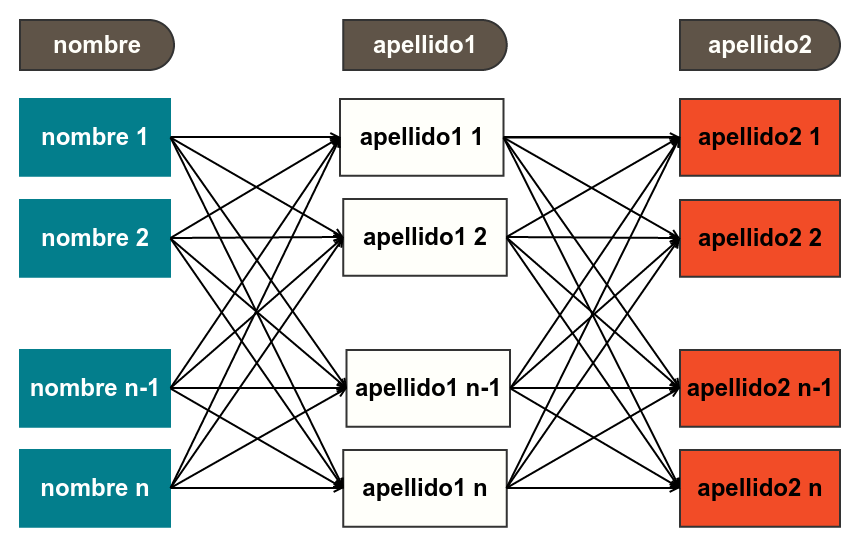
\includegraphics[scale=0.4]{images/listNameApe1Ape2.png}
\caption{Apartir de una lista de nombres}\label{fig:listNameLastName}
\end{figure}

\section{Tipos de datos binarios(Binary Data Types)}

Los sistemas gestores de base de datos(SGBD) permiten almacenar archivos en formatos como \texttt{bytea}, \texttt{blob} entre otros, variando estos segun el SGBD utilizado. 

En este proyecto se pondra a consideracion trabajar con postgresql el cual permite almacenar archivos en formato \texttt{bytea}. El tipo de dato \texttt{bytea} permite almacenar objetos de gran tama\~no, postgreSQL no conoce nada sobre el tipo de informaci\'on que se almacena \texttt{bytea}, simplemente lo considera como cadena binaria, Una cadena binaria es una secuencia de octetos (o bytes). 

Las cadenas binarias se distinguen de las cadenas de caracteres de dos maneras. En primer lugar, las cadenas binarias permiten espec\'ificamente el almacenamiento de octetos de valor cero y otros ``no imprimibles''  octetos (por lo general, octetos fuera comprendida entre 32 a 126). Las cadenas de caracteres no permite cero octetos, y tambi\'en no permite ning\'un otro valor de octeto y secuencias de valores de octeto que no son v\'alidos seg\'un la codificaci\'on  de caracteres seleccionado de la base de datos. En segundo lugar, las operaciones en cadenas binarias procesan los bytes reales, mientras que el procesamiento de cadenas de caracteres depende de la configuraci\'on regional. En resumen, las cadenas binarias son apropiadas para el almacenamiento de datos que el programador piensa como ``bytes en bruto'' , mientras que las cadenas de caracteres son apropiados para almacenar texto.

El tipo \texttt{bytea} soporta dos formatos externos de entrada y salida de formato ``escape'' y ``hex''. Ambos de estos siempre son aceptados en la entrada. El formato de salida depende del par\'ametro de configuraci\'on, el valor predeterminado es hexagonal. (Tenga en cuenta que el formato hexadecimal se introdujo en PostgreSQL 9.0. Versiones anteriores y algunas herramientas no lo entienden).

El SQL est\'andar define un tipo de cadena binaria diferente, llamado BLOB o de objeto binario grande . El formato de entrada es diferente de bytea , pero las funciones y operadores proporcionados son en su mayoría de la misma.
\subsection{Bytea formato hexadecimal}
El formato ``hex'' de datos binarios codifica como 2 d\'igitos hexadecimales por byte. Toda la cadena es precedido por la secuencia del signo barra contrario (para distinguirlo del formato de escape). En algunos contextos, puede ser necesario escapado con la duplicaci\'on de ella.
\subsection{Bytea escapar formato}
El formato ``escape'' es el tradicional formato de PostgreSQL para el tipo bytea.

A momento de generar datos de prueba para base de datos, el tipo de dato \texttt{bytea} llega a ser un caso especial, debido a que no es posible crearlo como cualquier otro dato, como ser un numero de tel'efono que llega a ser combinaciones de n'umeros bajo ciertas condiciones o el caso de un nombre que son combinaciones de vocales y consonantes, sin embargo \texttt{bytea} es posible generar haciendo uso de archivos existentes teniendo solo la ruta del archivo es suficiente para poder insertar en la base datos.
\section{Tipos fecha/hora}
\subsection{Generaci\'on de fechas}
Una fecha esta compuesta por tres partes:
\begin{itemize}
\item A\~no la parte del a\~no para nuestros d\'ias comprende de cuatro d\'igitos desde 1000 hasta el a\~no 9999 el rango no estrictamente establecido.
\item
Mes. la parte del mes se representa en n\'umero de dos d\'igitos que comprende en un rango establecido, con un inicio de 01 hasta 12 representando los doce meses del a\~no.
\item
 D\'ia. la cantidad de d\'ias en un mes es variable mucho depende a que mes se refiera, el rango comprende desde el d\'ia uno y con un final variable desde 28 a 31 d\'ias.
\end{itemize}
Para generar una cantidad de fechas es necesario tener una fecha inicial y final. a partir de ello se hace la combinacion cartesiana como se observa en la Figura \ref{fig:generacion de fechas}.
\begin{figure}[H]
\centering
\subfigure{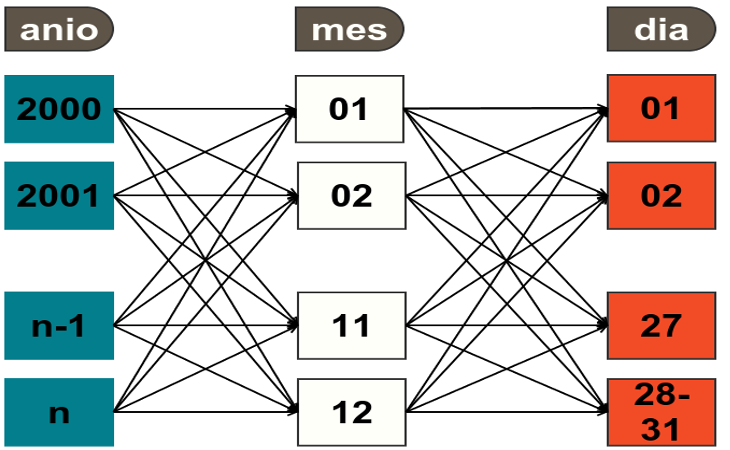
\includegraphics[scale=0.5]{images/algoritmoDates}}
\caption{Generaci'on de fechas} \label{fig:generacion de fechas}
\end{figure}
\subsubsection{Algoritmo de generaci\'on de fechas}
Para realizar la aplicaci\'on del algoritmo de generaci\'on de fechas es necesario tener dos datos una fecha inicial y otra fecha limite final donde es importante que la fecha inicial debe ser una fecha anterior a la final, la cantidad de fechas a obtener depender\'ia del tama\~no de rango que existe entre la inicial y la final.

A continuaci\'on se presenta el algoritmo \ref{alg:algoritmoGeneracionFechas} de generaci\'on de fechas en formato dd/mm/aa, tomando en cuenta que la cantidad de d\'ias es variable por cada mes adem\'as tomando en cuenta a\~nos bisiestos.
\begin{algorithm}[H]
\begin{algorithmic}[1]
\REQUIRE fechaInicio fechaFinal
\STATE fechas$[$ $]$
\STATE contador $\leftarrow$ 0
\IF{fechaInicio$ < $ fechaFinal}
	\WHILE {fechaInicio $<$ fechaFinal}
	\STATE fechas $[$ contador $]$ $\leftarrow$ fechaInicio+ 1 dia
	\STATE contador $\leftarrow$ contador+1
	\ENDWHILE
\ELSE
	\RETURN error
\ENDIF
\RETURN fechas
\end{algorithmic}
\caption{Algoritmo de generaci\'on de fechas}\label{alg:algoritmoGeneracionFechas}
\end{algorithm}
\subsection{Generaci\'on de dato tipo Time}
La estructura del dato tipo tiempo es muy similar a las fechas con la diferencia de que estas tienen un rango ya establecidos sin ninguna variaci\'on, esta compuesta por:
\begin{enumerate}
\item Hora. las hora se representa en un n\'umero de dos d\'igitos comenzando desde las 00 horas hasta las 23.
\item Minuto. los minutos tambi\'en se representa en un n\'umero de dos d\'igitos con un inicio en 00 hasta 59 minutos.
\item Segundo. el rango es id\'entica al de los minutos.
\end{enumerate}
Para generar el tipo de dato time se hace combinaciones de las tres partes que tiene este tipo de dato, realizando combinaciones se obtiene la cantidad de datos que requerida.

En la Figura \ref{fig:generacion de Time} se hace la combinaci\'on en modo cartesiano para la generaci\'on para este tipo de dato:

\begin{figure}[H]
\centering
\subfigure{\includegraphics[scale=0.3]{images/algoritmoTime}}
\caption{Generaci'on de Time} \label{fig:generacion de Time}
\end{figure}
\begin{algorithm}[H]
\begin{algorithmic}[1]
\REQUIRE fechaHoraInicio fechaHoraFinal
\STATE fechasHoras$[$ $]$
\STATE contador $\leftarrow$ 0
\IF{fechaHoraInicio$ < $ fechaHoraFinal}
	\WHILE {fechaHoraInicio $<$ fechaHoraFinal}
	\STATE fechasHoras $[$ contador $]$ $\leftarrow$ fechaHoraInicio+ 1 minuto
	\STATE contador $\leftarrow$ contador+1
	\ENDWHILE
\ELSE
	\RETURN error
\ENDIF
\RETURN fechasHoras
\end{algorithmic}
\caption{Algoritmo de generaci\'on de fecha hora}\label{alg:algoritmoGeneracionDateTime}
\end{algorithm}

\section{Tipos de direcciones de red}
Las direcciones de red que almacena una base de datos son la IPv4, IPv6 y direcci'on mac como se observa con mayor detalle en el cuadro \ref{tableredtipos}.
\begin{center}
\scriptsize
  \captionof{table}{Tipos de datos de red}
  \renewcommand{\arrayrulewidth}{1pt}
  \label{tableredtipos}
\begin{tabular}{|l|l|l|}
\hline
nombre  & tama\~no        & descripci\'on               \\ \hline
cidr    & 12 \'o 24 bytes & Redes IPv4 o IPv6         \\ \hline
inet    & 12 \'o 24 bytes & Hosts y redes IPv4 o IPv6 \\ \hline
macaddr & 6 bytes       & Direcci\'on MAC             \\ \hline
\end{tabular}
\end{center}
\subsection{Estructura de una direcci'on IPv4}
Al igual que la direcci\'on de una casa que tiene dos partes (una calle y un c'odigo postal), una direcci'on IP tambi'en est'a formada por dos partes: el ID de host y el ID de red.
\subsubsection{ID de red}
La primera parte de una direcci\'on IP es el ID de red, que identifica el segmento de red en el que est\'a ubicado el equipo.Todos los equipos del mismo segmento deben tener el mismo ID de red, al igual que las casas de una zona determinada tienen el mismo c\'odigo postal.
\subsubsection{ID de host}
La segunda parte de una direcci\'on IP es el ID de host, que identifica un equipo, un router u otro dispositivo de un segmento.El ID de cada host debe ser exclusivo en el ID de red, al igual que la direcci\'on de una casa es exclusiva dentro de la zona del c\'odigo postal. Es importante observar que al igual que dos zonas de c\'odigo postal distinto pueden tener direcciones iguales, dos equipos con diferentes IDs de red pueden tener el mismo ID de host. Sin embargo, la combinaci\'on del ID de red y el ID de host debe ser exclusivo para todos los equipos que se comuniquen entre s\'i. Las clases de direcciones se utilizan para asignar IDs de red a organizaciones para que los equipos de sus redes puedan comunicarse en Internet.

Para generar un dato de este tipo se puede hacer una combinaci'on cartesiana entre un rango de n'umeros entre 1 hasta 253 como se observa en la Figura \ref{fig:algoritmoGeneracionIPv4}.

\begin{figure}[H]
\centering
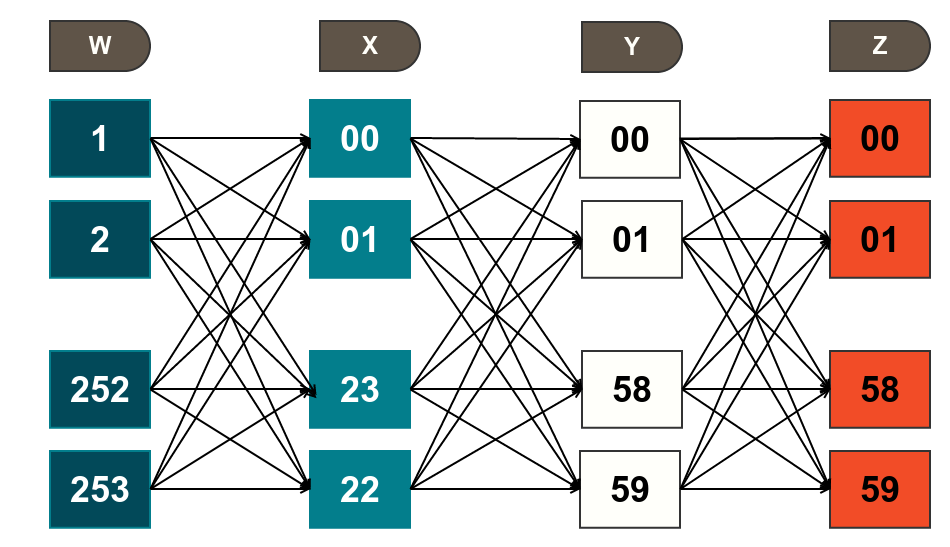
\includegraphics[scale=0.45]{images/ipv4.png}
\caption{Combinaci'on IPv4} \label{fig:algoritmoGeneracionIPv4}
\end{figure}

A continuaci'on se presenta el algoritmo \ref{alg:algoritmoGeneracionIPv4} para generar direcciones IPv4 para lo cual es necesario un dato de entrada de inicio y otra final.
\begin{algorithm}[H]
\begin{algorithmic}[1]
\REQUIRE inicio final
\STATE direcciones$[$ $]$
\STATE contador $\leftarrow$ 0
\IF{inicio$ < $ fiinal}
	\WHILE {inicio $<$ final}
	\STATE direcciones $[$ contador $]$ $\leftarrow$ inicio+ 1
	\STATE contador $\leftarrow$ contador+1
	\ENDWHILE
\ELSE
	\RETURN error
\ENDIF
\RETURN direcciones
\end{algorithmic}
\caption{Algoritmo de generaci\'on de IPv4}\label{alg:algoritmoGeneracionIPv4}
\end{algorithm}